\documentclass{beamer}
\usepackage[utf8]{inputenc}
\usepackage[UKenglish]{babel}
\usepackage[UKenglish]{isodate}
\usepackage{graphicx}
\usepackage{tikz}
\usepackage{phaistos}
\usepackage{wasysym}
\usepackage{listings}
\usepackage[lighttt]{lmodern}
\usepackage{xcolor}

\usetikzlibrary{shapes,calc}
\tikzstyle{na} = [baseline=-0.5ex]
\tikzstyle{every picture}+=[remember picture]

\usetheme{Boadilla}
\beamertemplatenavigationsymbolsempty
\author{Paulius Dilkas}
\title[Nondeterministic Bigraphs]{Nondeterministic Bigraphs and Their Use in
  Modelling Movement}
%s\subtitle{}
\institute[]{Formal Analysis, Theory and Algorithms}
\date{16th October 2018}

\newcommand\pro{\item[\textcolor{green}{$+$}]}
\newcommand\con{\item[\textcolor{red}{$-$}]}
\providecommand\longdoublearrowRHD{\mathrel\LHD\joinrel\relbar\joinrel\relbar\joinrel\mathrel\RHD}
\providecommand\longrightarrowRHD{\relbar\joinrel\relbar\joinrel\mathrel\RHD}
\makeatletter
\providecommand*\xrightarrowRHD[2][]{\ext@arrow 0055{\arrowfill@\relbar\relbar\longrightarrowRHD}{#1}{#2}}
\makeatother

\definecolor{keyword}{HTML}{008000}
\definecolor{comment}{HTML}{408080}
\definecolor{name}{HTML}{BA2121}
\definecolor{operator}{HTML}{AA22FF}

\lstdefinelanguage{Big}{
  basicstyle=\ttfamily,
  sensitive=true,
  morekeywords={fun, brs, end, sbrs, pbrs, nbrs, begin, init, atomic, preds,
    rules, action, big, ctrl, float, int, react, id},
  comment=[l]{\#},
  keywordstyle=\bfseries\color{keyword},
  commentstyle=\itshape\color{comment},
  alsoletter={=,|,-,>,@},
  emph={=,|,||,-,->,-->,@},
  emphstyle=\color{operator},
}

\lstset{language=Big}

\ttfamily
\DeclareFontShape{OT1}{lmtt}{m}{it}
     {<->sub*lmtt/m/sl}{}

\begin{document}
\maketitle

\begin{frame}{Motivation}
  \begin{columns}[t]
    \column{0.5\textwidth}
    \centering
    \begin{overlayarea}{\textwidth}{0.5\textheight}
      \includegraphics<-2>[width=\textwidth]{uav.jpg}
      \includegraphics<3->[width=\textwidth]{drone.jpg}
    \end{overlayarea}
    \begin{overlayarea}{\textwidth}{0.5\textheight}
      \includegraphics<-3>[width=\textwidth]{underwater.jpg}
      \includegraphics<4->[width=\textwidth]{boat.png}
    \end{overlayarea}
    \column{0.5\textwidth}
    \centering
    \begin{overlayarea}{\textwidth}{0.5\textheight}
      \includegraphics<1>[width=\textwidth]{ground.jpg}
      \includegraphics<2->[width=\textwidth]{car.jpg}
    \end{overlayarea}
    \includegraphics[width=\textwidth]{rover.jpg}
  \end{columns}
\end{frame}

\begin{frame}{Markov Decision Process}
  \begin{figure}
    \centering
    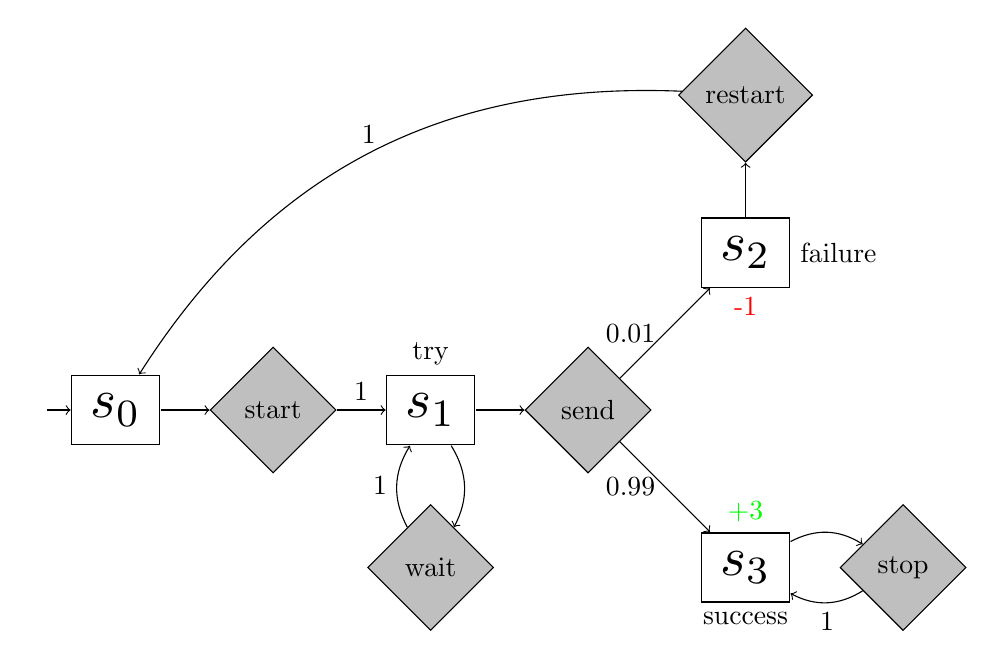
\begin{tikzpicture}[state/.style={rectangle, draw, scale=2},
      action/.style={diamond, draw, fill=lightgray, minimum size=1.6cm}]
      \node(origin) at (-1, 0){};
      \node[state](s0) at (0, 0){$s_0$};
      \node[action](start) at (2, 0){start};
      \node[state,label=try](s1) at (4, 0){$s_1$};
      \node[action](wait) at (4, -2){wait};
      \node[action](send) at (6, 0){send};
      \node[state,label={right:failure},label={below:\textcolor{red}{-1}}](s2) at (8, 2){$s_2$};
      \node[action](restart) at (8, 4){restart};
      \node[state,label={below:success},label={above:\textcolor{green}{+3}}](s3) at (8, -2){$s_3$};
      \node[action](stop) at (10, -2){stop};
      \draw[-{>[scale=2]}] (s0) edge (start);
      \draw[-{>[scale=2]}] (start) edge node[above] {$1$} (s1);
      \draw[-{>[scale=2]},bend left] (s1) edge (wait);
      \draw[-{>[scale=2]},bend left] (wait) edge node[left] {$1$} (s1);
      \draw[-{>[scale=2]}] (s1) edge (send);
      \draw[-{>[scale=2]}] (send) edge node[left] {$0.01$} (s2);
      \draw[-{>[scale=2]}] (send) edge node[left] {$0.99$} (s3);
      \draw[-{>[scale=2]}] (s2) edge (restart);
      \draw[-{>[scale=2]},bend right] (restart) edge node[above] {$1$} (s0);
      \draw[-{>[scale=2]},bend left] (s3) edge (stop);
      \draw[-{>[scale=2]},bend left] (stop) edge node[below] {$1$} (s3);
      \draw[-{>[scale=2]}] (origin) edge (s0);
    \end{tikzpicture}
  \end{figure}
\end{frame}

\begin{frame}{Collecting Objects in a Grid}
  \begin{itemize}
  \item Each cell is either visited or unvisited.
    \pause
  \item When entering an unvisited cell, with probability $p$ the agent receives
    an object.
    \pause
  \item Once a set number of objects is collected, the agent heads home.
  \end{itemize}
\end{frame}

\begin{frame}{Collecting Objects in a Grid}
  \begin{figure}
    \centering
    \begin{tikzpicture}[overlay]
      \only<1>{
        \fill[fill=black!20!white] (-1, -2) rectangle (2, 2);
        \fill[fill=black!20!white] (-2, -1) rectangle (-1, 2);
        \draw[step=1cm,very thin] (-2, -2) grid (2, 2);
        \node at (-1.5, -1.6) {\PHchild};
      }
      \only<2>{
        \fill[fill=black!20!white] (-1, -2) rectangle (2, 2);
        \fill[fill=black!20!white] (-2, 0) rectangle (-1, 2);
        \draw[step=1cm,very thin] (-2, -2) grid (2, 2);
        \node at (-1.5, -0.6) {\PHchild};
      }
      \only<3>{
        \fill[fill=black!20!white] (-1, -2) rectangle (2, 2);
        \fill[fill=black!20!white] (-2, 1) rectangle (-1, 2);
        \draw[step=1cm,very thin] (-2, -2) grid (2, 2);
        \node at (-1.4, 0.4) {\PHchild};
        \node at (-1.8, 0.4) {$\bigstar$};
      }
      \only<4>{
        \fill[fill=black!20!white] (-1, -2) rectangle (2, 2);
        \fill[fill=black!20!white] (-2, 1) rectangle (-1, 2);
        \draw[step=1cm,very thin] (-2, -2) grid (2, 2);
        \node at (-1.4, -0.6) {\PHchild};
        \node at (-1.8, -0.6) {$\bigstar$};
      }
      \only<5>{
        \fill[fill=black!20!white] (0, -2) rectangle (2, 2);
        \fill[fill=black!20!white] (-2, 1) rectangle (-1, 2);
        \fill[fill=black!20!white] (-1, 0) rectangle (0, 2);
        \fill[fill=black!20!white] (-1, -2) rectangle (0, -1);
        \draw[step=1cm,very thin] (-2, -2) grid (2, 2);
        \node at (-0.4, -0.6) {\PHchild};
        \node at (-0.8, -0.8) {$\bigstar$};
        \node at (-0.8, -0.5) {$\bigstar$};
      }
      \only<6>{
        \fill[fill=black!20!white] (0, -2) rectangle (2, 2);
        \fill[fill=black!20!white] (-2, 1) rectangle (-1, 2);
        \fill[fill=black!20!white] (-1, 0) rectangle (0, 2);
        \fill[fill=black!20!white] (-1, -2) rectangle (0, -1);
        \draw[step=1cm,very thin] (-2, -2) grid (2, 2);
        \node at (-1.4, -0.6) {\PHchild};
        \node at (-1.8, -0.8) {$\bigstar$};
        \node at (-1.8, -0.5) {$\bigstar$};
      }
      \only<7>{
        \fill[fill=black!20!white] (0, -2) rectangle (2, 2);
        \fill[fill=black!20!white] (-2, 1) rectangle (-1, 2);
        \fill[fill=black!20!white] (-1, 0) rectangle (0, 2);
        \fill[fill=black!20!white] (-1, -2) rectangle (0, -1);
        \draw[step=1cm,very thin] (-2, -2) grid (2, 2);
        \node at (-1.4, -1.6) {\PHchild};
        \node at (-1.8, -1.8) {$\bigstar$};
        \node at (-1.8, -1.5) {$\bigstar$};
      }
    \end{tikzpicture}
  \end{figure}
\end{frame}

\begin{frame}{A High Level View}
  \begin{itemize}
  \item Controls (types of nodes)
    \pause
    \begin{itemize}
    \item \texttt{Agent, Cell, Directions, Object}
      \pause
    \item \texttt{North, East, West, South}
      \pause
    \item \texttt{Visited, Unvisited}
    \end{itemize}
    \pause
  \item Predicates (properties to check)
    \begin{itemize}
    \item \texttt{goal}: collected the required number of objects
    \item \texttt{home}: is in the southwest corner of the grid
    \end{itemize}
    \pause
  \item Reaction rules (how the state changes)
    \pause
    \begin{itemize}
    \item Grouped into \alert{actions} by direction
    \item Different rules for going to visited and unvisited cells
      \pause
    \item Priority 1: going/staying home (5 rules)
      \pause
    \item Priority 2: 3 rules for each direction
      \begin{itemize}
      \item visited
      \item unvisited
      \item unvisited + object
      \end{itemize}
    \end{itemize}
  \end{itemize}
\end{frame}

\begin{frame}[t]{Transition System}
  \begin{tikzpicture}[overlay]
    \node () at (7.5, -3.8) {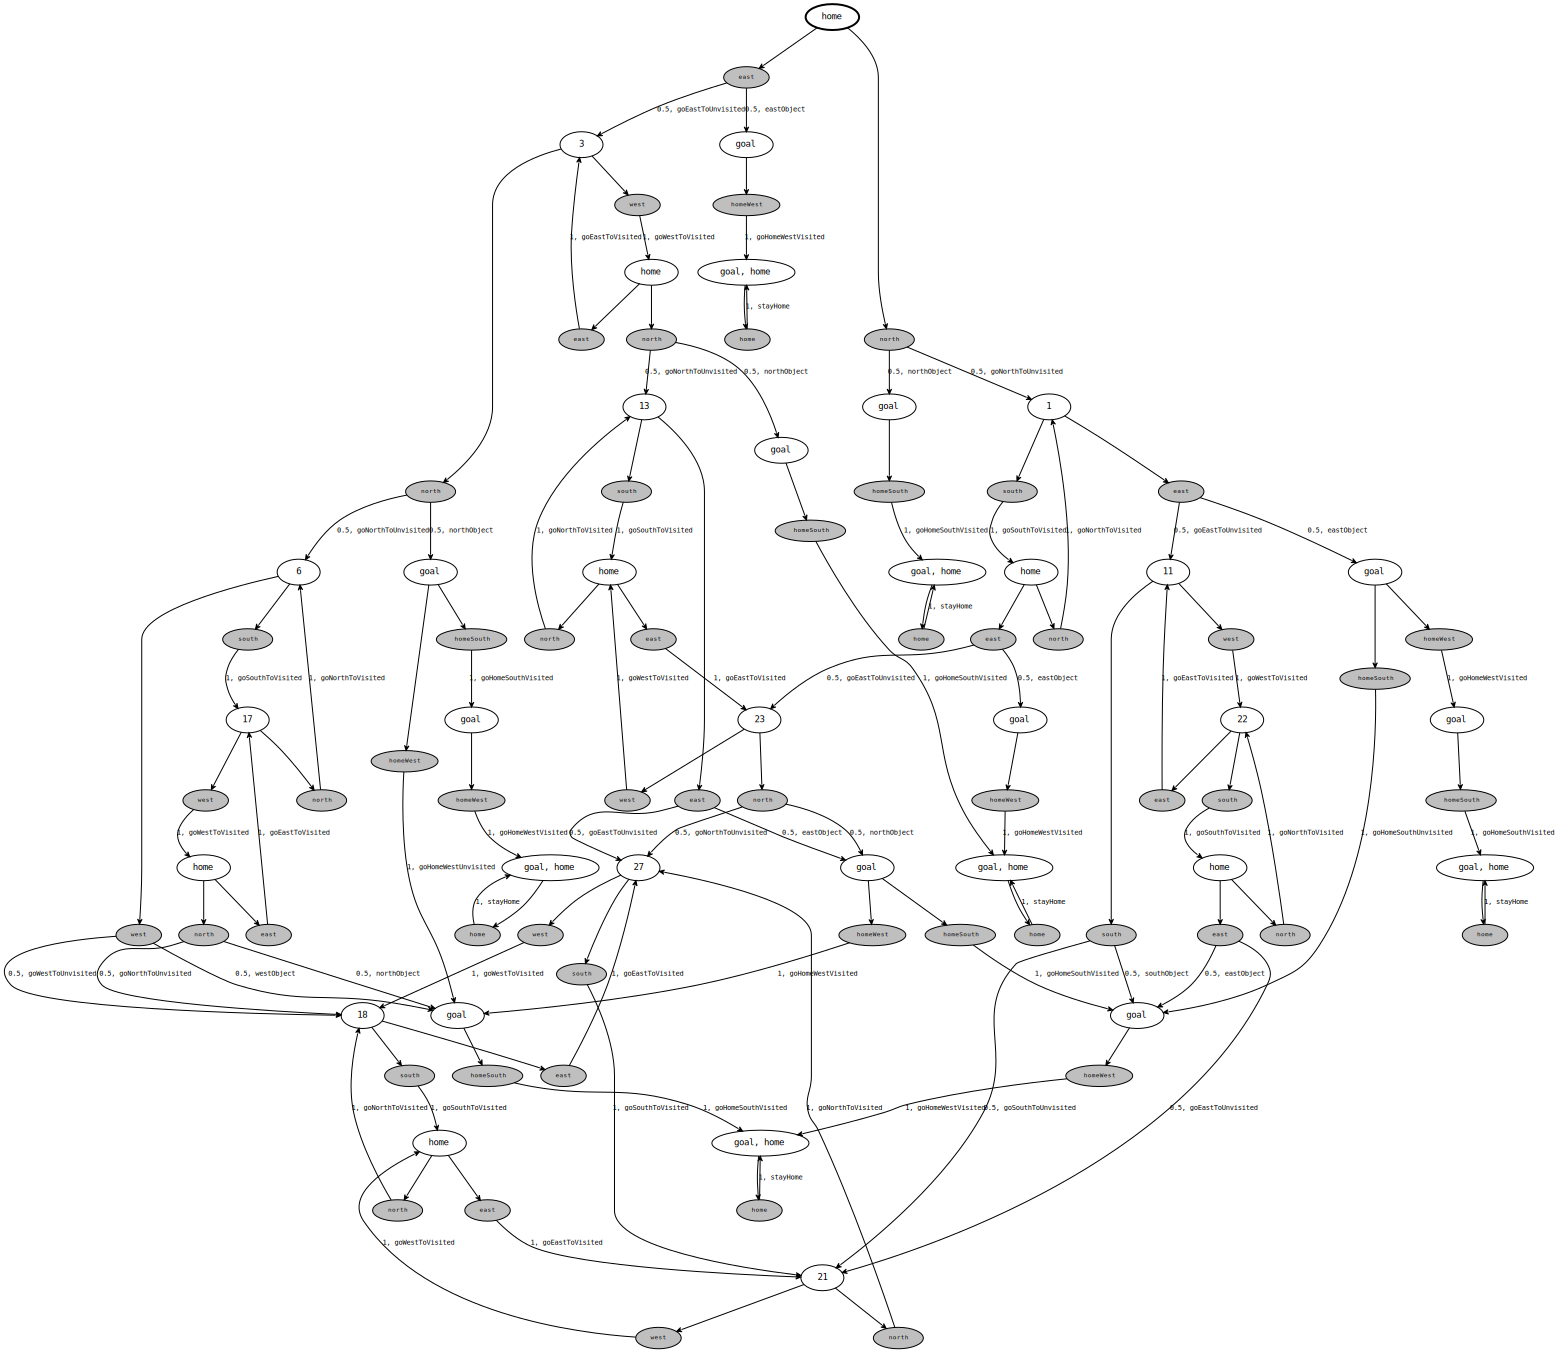
\includegraphics[clip, trim=15cm 35.2cm 20cm 0cm, width=\textwidth]{../models/agent1/ts.pdf}};
    \path[->]<2-5> (t-state) edge[blue] (9.5, -0.4);
    \path[->,bend left=10]<3-5> (t-action) edge[blue] (7.8, -1.5);
    \path[->]<4-5> (t-rules) edge[blue] (6.4, -2.2);
    \path[->,bend left=10]<4-5> (t-rules) edge[blue] (8.3, -2.2);
    \path[->]<5> (t-predicate) edge[blue] (8, -3);
  \end{tikzpicture}
  \begin{itemize}
  \item<2-6> States \tikz[na] \coordinate (t-state);
  \item<3-6> Actions \tikz[na] \coordinate (t-action);
  \item<4-6> Reaction rules with probabilities \tikz[na] \coordinate (t-rules);
  \item<5-6> Predicates \tikz[na] \coordinate (t-predicate);
  \end{itemize}
\end{frame}

\begin{frame}{Transition System}
  \begin{figure}
    \centering
    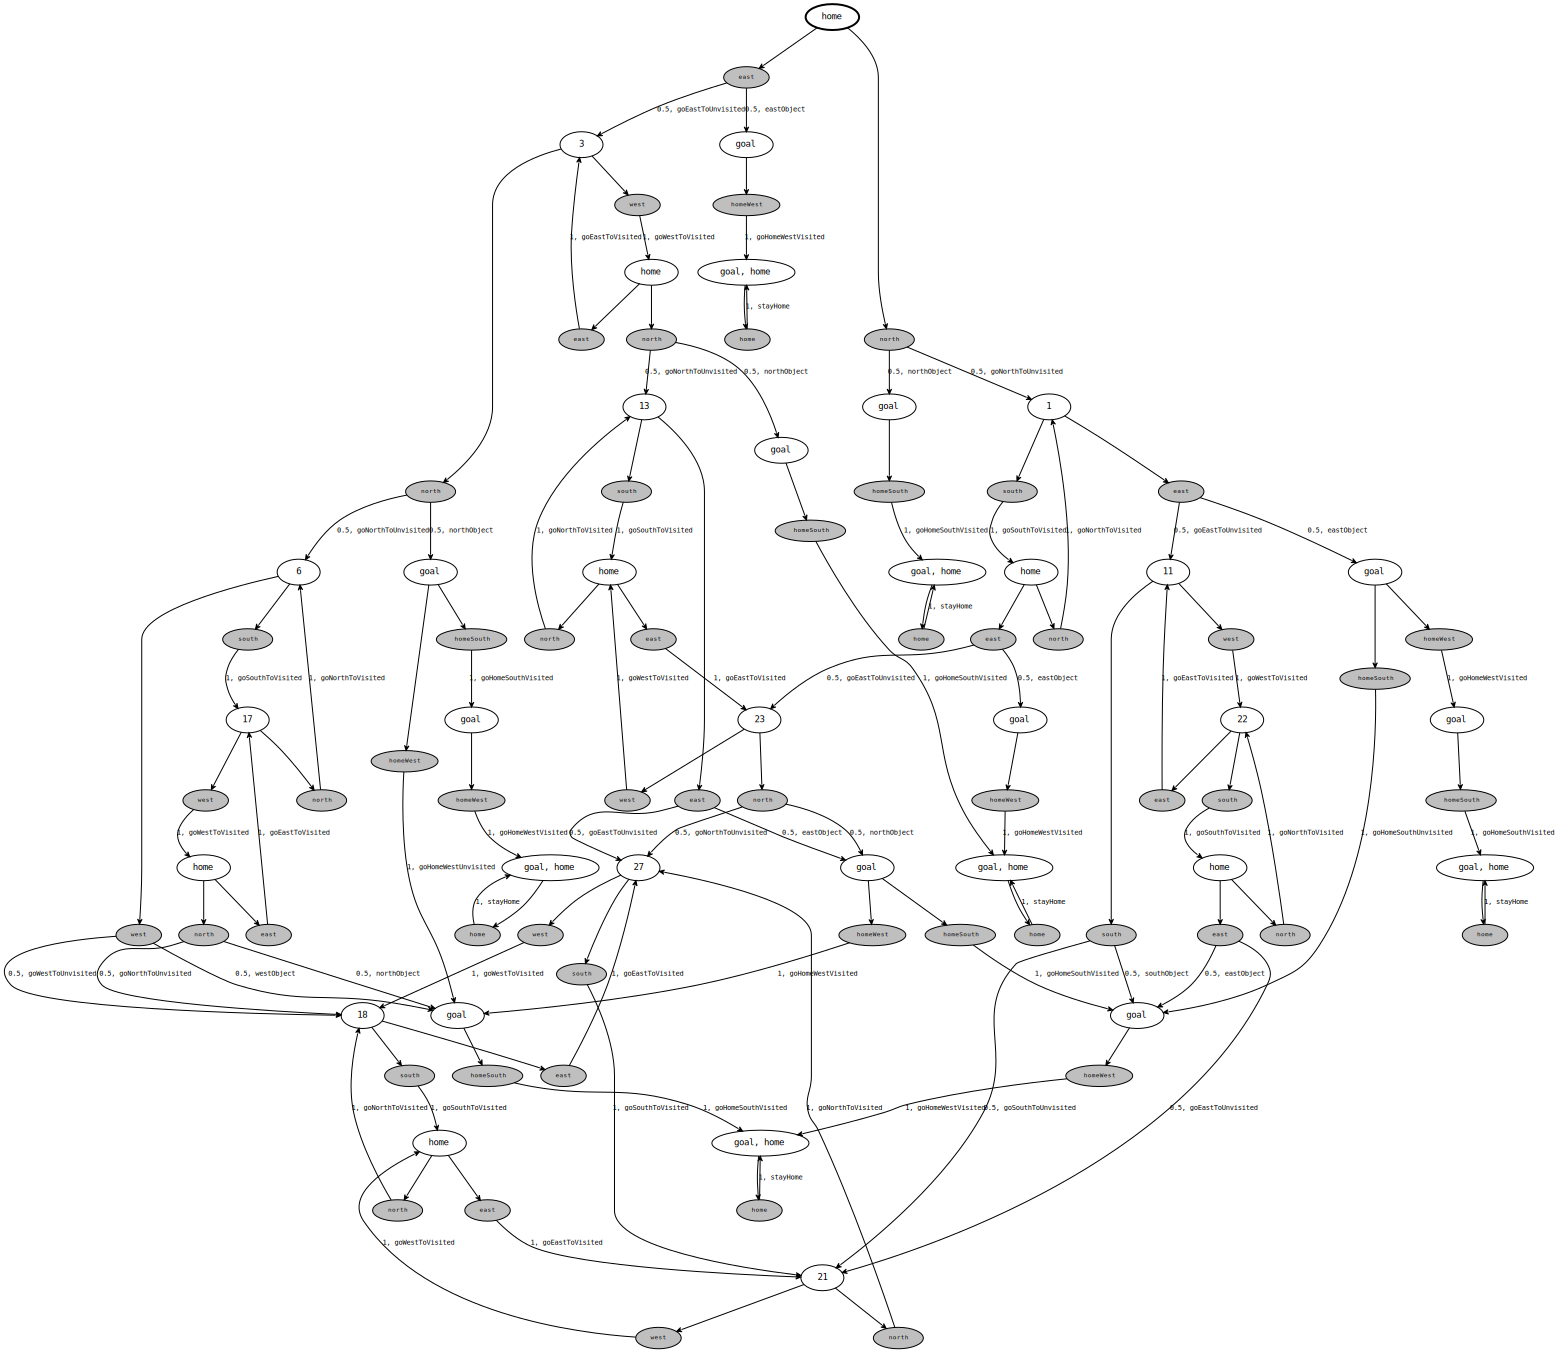
\includegraphics[scale=0.17]{../models/agent1/ts.pdf}
  \end{figure}
\end{frame}

\begin{frame}{The Workflow}
  \begin{itemize}
  \item Start with an initial state
    \pause
  \item Find all applicable reaction rules (from the highest non-empty priority
    class)
    \begin{itemize}
    \item Priorities and actions are orthogonal concepts
    \end{itemize}
    \pause
  \item Normalise probabilities per action
    \pause
    \begin{itemize}
    \item Caveat: one rule can sometimes be applied in multiple ways
    \item In that case, each outcome is equally likely
    \end{itemize}
    \pause
  \item Either:
    \begin{itemize}
    \item Breadth first search to generate the full transition system
    \item Or select the next state randomly for a simulation
    \end{itemize}
  \end{itemize}
\end{frame}

\begin{frame}{Bigraphs}
  \lstset{morecomment=[s][\color{name}]{\{}{\}}}
  \begin{columns}
    \begin{column}{0.5\textwidth}
      \only<-5>{
        \begin{itemize}
        \item<2-> Region \tikz[na] \coordinate (t-region);
        \item<3-> Nodes \tikz[na] \coordinate (t-node);
        \item<4-> Site \tikz[na] \coordinate (t-site);
        \item<5-> Links \tikz[na] \coordinate (t-link);
        \end{itemize}
      }
    \end{column}
    \begin{column}{0.5\textwidth}
      \begin{figure}
        \centering
        \begin{tikzpicture}
          \node {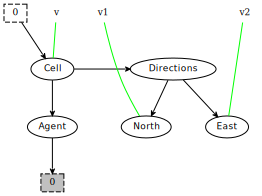
\includegraphics[width=\textwidth]{../models/agent1/home.pdf}};
          \path (-3, 1.9) coordinate (region);
          \path (-2.4, 0.7) coordinate (node1);
          \path (-2.4, -0.5) coordinate (node2);
          \path (-2.2, -1.8) coordinate (site);
          \path (-1.9, 2.1) coordinate (link1);
          \path (-0.8, 2.1) coordinate (link2);
          \path (2.5, 2.1) coordinate (link3);
        \end{tikzpicture}
      \end{figure}
    \end{column}
  \end{columns}
  \onslide<6>{
    \lstinputlisting[firstline=16, lastline=18,
    xleftmargin=0.09\textwidth]{../models/agent1/agent.big}
  }
  \begin{tikzpicture}[overlay]
    \path[->]<2-5> (t-region) edge[blue] (region);
    \path[->]<3-5> (t-node) edge[blue] (node1);
    \path[->]<3-5> (t-node) edge[blue] (node2);
    \path[->]<4-5> (t-site) edge[blue] (site);
    \path[->,bend left=60]<5> (t-link) edge[blue] (link1);
    \path[->,bend left=70]<5> (t-link) edge[blue] (link2);
    \path[->,bend left=80]<5> (t-link) edge[blue] (link3);
  \end{tikzpicture}
\end{frame}

\begin{frame}[fragile]{Initial State}
\lstset{morecomment=[s][\color{name}]{\{}{\}}}
\begin{lstlisting}

big initial = Visited{v}
           || Unvisited{u}
           # bottom left
           || Cell{v}.(Directions.(North{a}
                                 | East{b})
                     | Agent.1)
           # top left
           || Cell{u}.Directions.(East{c}
                                | South{a})
           # bottom right
           || Cell{u}.Directions.(North{d}
                                | West{b})
           # top right
           || Cell{u}.Directions.(West{c}
                                | South{d});

\end{lstlisting}
\end{frame}

\begin{frame}{Reaction Rule: Go West and Collect an Object}
  \begin{columns}
    \begin{column}{0.45\textwidth}
      \begin{figure}
        \centering
        \includegraphics[width=\textwidth]{../models/agent1/westObject_lhs.pdf}
      \end{figure}
    \end{column}
    \begin{column}{0.1\textwidth}
      $\xrightarrowRHD{p}$
    \end{column}
    \begin{column}{0.45\textwidth}
      \begin{figure}
        \centering
        \includegraphics[width=\textwidth]{../models/agent1/westObject_rhs.pdf}
      \end{figure}
    \end{column}
  \end{columns}
\end{frame}

\begin{frame}{A Tale of Schr\"{o}dinger's Wall...}
  \begin{figure}
    \centering
    \includegraphics[height=\textheight]{schrodinger.jpg}
  \end{figure}
\end{frame}

\begin{frame}{A Tale of Schr\"{o}dinger's Wall...}
  \begin{figure}
    \centering
    
\begin{tikzpicture}[overlay]
      \only<1>{
        % outside walls
        \draw (-0.25, 0.5) -- (-1.5, 0.5) -- (-1.5, 1.5) -- (1.5, 1.5) -- (1.5, 0.5) -- (0.25, 0.5);
        % background grid
        \draw[gray,very thin] (-0.5, 1.5) -- (-0.5, 0.5);
        \draw[gray,very thin] (0.5, 1.5) -- (0.5, 0.5);
        % agent
        \node at (-1, 0.9) {\PHchild};
        % door
        \draw[brown,ultra thick] (-0.25, 0.5) -- (0.25, 0.5);
      }
      \only<2>{
        % outside walls
        \draw (-0.25, 0.5) -- (-1.5, 0.5) -- (-1.5, 1.5) -- (1.5, 1.5) -- (1.5, 0.5) -- (0.25, 0.5);
        % background grid
        \draw[gray,very thin] (-0.5, 1.5) -- (-0.5, 0.5);
        \draw[gray,very thin] (0.5, 1.5) -- (0.5, 0.5);
        % agent
        \node at (0, 0.9) {\PHchild};
        % door
        \draw[brown,ultra thick] (-0.25, 0.5) -- (0.25, 0.5);
      }
      \only<3-4>{
        % outside walls
        \draw (1.5, 0.5) -- (1.5, -1.5) -- (-0.5, -1.5) -- (-0.5, 0.5) -- (-1.5, 0.5) -- (-1.5, 1.5) -- (1.5, 1.5) -- (1.5, 0.5) -- (0.5, 0.5);
        % probabilistic wall
        \draw[red,ultra thick,dashed] (0.5, 0.5) -- (0.5, -0.5);
        % background grid
        \draw[gray,very thin] (-0.5, 1.5) -- (-0.5, 0.5);
        \draw[gray,very thin] (0.5, 1.5) -- (0.5, 0.5);
        \draw[gray,very thin] (-0.5, -0.5) -- (1.5, -0.5);
        \draw[gray,very thin] (0.5, -0.5) -- (0.5, -1.5);
        % agent
        \node at (0, 0.9) {\PHchild};
        % door
        \draw[dotted] (-0.25, 0.5) arc (180:270:0.5cm);
        \draw[brown,ultra thick] (0.25, 0) -- (0.25, 0.5) node[right,  near start]{};
        \draw (-0.5, 0.5) -- (-0.25, 0.5);
        \draw (0.25, 0.5) -- (0.5, 0.5);
        % target
        \node at (1, 0) {$\bigstar$};
      }
      \only<4>{
        \draw[->, ultra thick, green] (0, 0.5) -- (0, 0) -- (0.8, 0);
        \draw[->, ultra thick, green] (0, 0.5) -- (0, -1) -- (1, -1) -- (1, -0.2);
      }
    \end{tikzpicture}
  \end{figure}
\end{frame}

\begin{frame}{A High Level View}
  \begin{itemize}
  \item Controls
    \begin{itemize}
    \item \texttt{Agent, Cell, Directions, \alert{Goal}, \alert{Node}}
      \pause
    \item \texttt{North, East, West, South}
    \item no \texttt{Object}, no \texttt{Visited/Unvisited}
    \end{itemize}
    \pause
  \item Reaction rules
    \begin{itemize}
    \item Priority 1: generating the room (2 rules in 1 action)
      \pause
    \item Priority 2: movement in 6 directions (including going in/out)
      \begin{itemize}
      \item each rule in a separate action
      \end{itemize}
    \end{itemize}
    \pause
  \item Predicate
    \begin{itemize}
    \item is \texttt{Agent} and \texttt{Goal} in the same cell?
    \end{itemize}
  \end{itemize}
\end{frame}

\begin{frame}{The Main Idea}
  \begin{columns}
    \begin{column}{0.5\textwidth}
      \begin{itemize}
      \item<2-> Outside the door \tikz[na] \coordinate (t-outside);
      \item<3-> The room \tikz[na] \coordinate (t-room);
      \item<4-> Inside the door \tikz[na] \coordinate (t-inside);
      \item<5-> Which cell is closest to the \tikz[na] \coordinate (t-link);
        door?
      \end{itemize}
    \end{column}
    \begin{column}{0.5\textwidth}
      \begin{figure}
        \begin{tikzpicture}
          \node {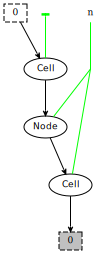
\includegraphics{../models/agent2/nesting_example/example.pdf}};
          \path (-1, 1.1) coordinate (outside);
          \path (-1, -0.8) coordinate (room);
          \path (0, -2.7) coordinate (inside);
          \path (1.4, 1.1) coordinate (link);
        \end{tikzpicture}
      \end{figure}
    \end{column}
  \end{columns}
  \begin{tikzpicture}[overlay]
    \path[->]<2-> (t-outside) edge[blue] (outside);
    \path[->]<3-> (t-room) edge[blue] (room);
    \path[->,bend left=20]<4-> (t-inside) edge[blue] (inside);
    \path[->,bend right=10]<5-> (t-link) edge[blue] (link);
  \end{tikzpicture}
\end{frame}

\begin{frame}{Initial State}
  \begin{figure}
    \centering
    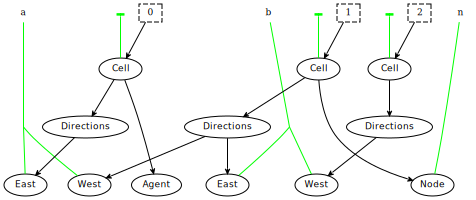
\includegraphics[width=\textwidth]{../models/agent2/initial.pdf}
  \end{figure}
\end{frame}

\begin{frame}{Opening the Door}
  \begin{figure}
    \centering
    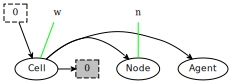
\includegraphics{../models/agent2/closedDoor_lhs.pdf}
  \end{figure}
\end{frame}

\begin{frame}{Opening the Door}
  \begin{figure}
    \centering
    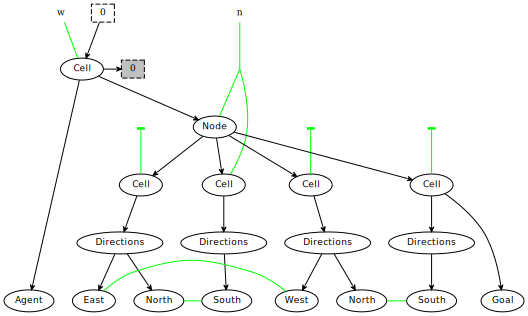
\includegraphics[width=\textwidth]{../models/agent2/closedDoor_rhs.pdf}
  \end{figure}
\end{frame}

\begin{frame}{Entering/Leaving a Room}
  \begin{columns}
    \begin{column}{0.45\textwidth}
      \begin{figure}
        \centering
        \includegraphics[width=\textwidth]{../models/agent2/goIn_lhs.pdf}
      \end{figure}
    \end{column}
    \begin{column}{0.1\textwidth}
      $\longdoublearrowRHD$
    \end{column}
    \begin{column}{0.45\textwidth}
      \begin{figure}
        \centering
        \includegraphics[width=\textwidth]{../models/agent2/goIn_rhs.pdf}
      \end{figure}
    \end{column}
  \end{columns}
\end{frame}

\begin{frame}[fragile]{Entering/Leaving a Room}
  \lstset{morecomment=[s][\color{name}]{\{}{\}}}
  \onslide<2>{Action rewards \tikz[na] \coordinate (text);}
  \begin{onlyenv}<1>
\begin{lstlisting}

action goIn
  react goIn = Cell{x}.(Agent | Node{n}.(Cell{n}
                                       | id)
                      | id)
               -[1.0]->
               Cell{x}.(Node{n}.(Cell{n}.(Agent
                                        | id)
                               | id)
                      | id);
end

\end{lstlisting}
  \end{onlyenv}
  \begin{onlyenv}<2>
\begin{lstlisting}[escapechar=!]

action goIn!\alert{[1]}!
  react goIn = Cell{x}.(Agent | Node{n}.(Cell{n}
                                       | id)
                      | id)
               -[1.0]->
               Cell{x}.(Node{n}.(Cell{n}.(Agent
                                        | id)
                               | id)
                      | id);
end

\end{lstlisting}
  \end{onlyenv}
  \onslide<2>{
    \begin{tikzpicture}[overlay]
      \path[->] (text) edge[blue] (2.9, 5.3);
    \end{tikzpicture}
  }
\end{frame}

\begin{frame}[fragile]{Tracking Time with State Rewards}
  \begin{columns}
    \begin{column}{0.5\textwidth}
\begin{lstlisting}[escapechar=!]

!\tikz{\coordinate (blanket-1)}!big agent = Agent;!\tikz{\coordinate (blanket-2)}!

begin !\tikz{\coordinate (nbrs-1)}!nbrs!\tikz{\coordinate (nbrs-2)}!
  init !\tikz{\coordinate (init-1)}!initialState!\tikz{\coordinate (init-2)}!;
  rules = !\tikz{\coordinate (rules-1)}![ {...}, {...} ]!\tikz{\coordinate (rules-2)}!;
  preds = !\tikz{\coordinate (preds-1)}!{ agent!\tikz{\coordinate (reward-1)}![1]!\tikz{\coordinate (reward-2)}! }!\tikz{\coordinate (preds-2)}!;
end

\end{lstlisting}
    \end{column}
    \begin{column}{0.5\textwidth}
      \begin{itemize}
      \item<2-> Blanket predicate
      \item<3-> Nondeterministic Bigraphical Reactive System
      \item<4-> Initial state
      \item<5-> List of reaction rules (grouped into priority classes)
      \item<6-> List of predicates
      \item<7-> Predicate rewards (optional)
      \end{itemize}
    \end{column}
  \end{columns}
  \begin{tikzpicture}[overlay]
    \draw<2> [red,thick] let \p1 = (blanket-1) in let \p2 = (blanket-2) in (\x1,\y1-1ex) rectangle (\x2, \y2+2ex);
    \draw<3> [red,thick] let \p1 = (nbrs-1) in let \p2 = (nbrs-2) in (\x1,\y1-1ex) rectangle (\x2, \y2+2ex);
    \draw<4> [red,thick] let \p1 = (init-1) in let \p2 = (init-2) in (\x1,\y1-1ex) rectangle (\x2, \y2+2ex);
    \draw<5> [red,thick] let \p1 = (rules-1) in let \p2 = (rules-2) in (\x1,\y1-1ex) rectangle (\x2, \y2+2ex);
    \draw<6> [red,thick] let \p1 = (preds-1) in let \p2 = (preds-2) in (\x1,\y1-1ex) rectangle (\x2, \y2+2ex);
    \draw<7> [red,thick] let \p1 = (reward-1) in let \p2 = (reward-2) in (\x1,\y1-1ex) rectangle (\x2, \y2+2ex);
  \end{tikzpicture}
\end{frame}

\begin{frame}{Extensions}
  \begin{itemize}
  \item Multiple rooms (make each \texttt{Node} uniquely identifiable)
    \pause
  \item Arbitrarily complex configurations (via bigraphs with sharing)
  \end{itemize}
  \begin{columns}
    \begin{column}{0.5\textwidth}
      \begin{figure}
        \centering
        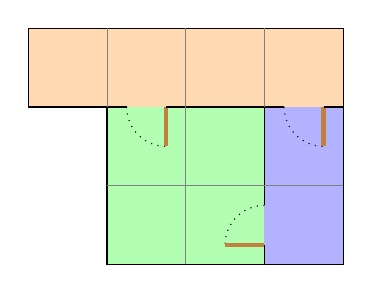
\begin{tikzpicture}
          % background colours
          \fill [orange!30] (0, 2) rectangle (4, 3);
          \fill [green!30] (1, 0) rectangle (3, 2);
          \fill [blue!30] (3, 0) rectangle (4, 2);
          % outer walls
          \draw (4, 2) -- (4, 0) -- (1, 0) -- (1, 2) -- (0, 2) -- (0, 3) -- (4, 3) -- (4, 2);
          % inner walls
          \draw (2, 2) -- (3, 2) -- (3, 1);
          % door 1
          \draw[dotted] (1.25,2) arc (180:270:0.5cm);
          \draw[brown,ultra thick] (1.75,1.5) -- (1.75,2) node[right,  near start]{};
          \draw (1, 2) -- (1.25, 2);
          \draw (1.75, 2) -- (2, 2);
          % door 2
          \draw[dotted] (3.25,2) arc (180:270:0.5cm);
          \draw[brown,ultra thick] (3.75,1.5) -- (3.75,2) node[right,  near start]{};
          \draw (3, 2) -- (3.25, 2);
          \draw (3.75, 2) -- (4, 2);
          % door 3
          \draw[dotted] (3, 0.75) arc (90:180:0.5cm);
          \draw[brown,ultra thick] (2.5, 0.25) -- (3, 0.25) node[right,  near start]{};
          \draw (3, 0.25) -- (3, 0);
          \draw (3, 0.75) -- (3, 1);
          % background grid
          \draw[gray,very thin] (1, 3) -- (1, 2);
          \draw[gray,very thin] (2, 3) -- (2, 0);
          \draw[gray,very thin] (3, 3) -- (3, 2);
          \draw[gray,very thin] (1, 1) -- (4, 1);
        \end{tikzpicture}
      \end{figure}
    \end{column}
    \pause
    \begin{column}{0.5\textwidth}
      \begin{figure}
        \centering
        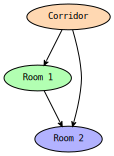
\includegraphics{multiple_rooms.pdf}
      \end{figure}
    \end{column}
  \end{columns}
  \pause
  \begin{tikzpicture}[overlay]
    \path[->,bend left=10] (2.6, 3) edge[blue,thick] (9, 4);
    \path[->,bend left=10] (4.6, 3) edge[blue,thick] (9.9, 3.5);
    \path[->,bend left=10] (3.6, 1.6) edge[blue,thick] (8.9, 1.8);
  \end{tikzpicture}
\end{frame}

\begin{frame}{Limitations of the Model}
  \begin{itemize}
  \item One door per cell
    \begin{itemize}
    \item Otherwise which door the agent uses would be random
      \pause
    \item Workaround: use more cells
    \end{itemize}
    \pause
  \item Two ideas in one: discovering space \& entering an inner space
  \end{itemize}
\end{frame}

\begin{frame}{A New Interface}
  \begin{figure}
    \centering
    \includegraphics{screenshot.jpg}
  \end{figure}
\end{frame}

\begin{frame}{A New Interface}
  \begin{itemize}
  \item Similar workflow to other Jupyter notebooks
  \item<2-> Syntax highlighting
  \item<3-> Visualisation of bigraphs and reaction rules
  \item<4-> Full and partial transition diagrams
    \begin{itemize}
    \item with state bigraph preview on mouseover
    \end{itemize}
  \item<5-> Backwards compatible to run OCaml code
  \end{itemize}
  \begin{block}{Available at}
    \url{https://github.com/dilkas/bigrapher-jupyter}
  \end{block}
\end{frame}

% exporting to prism: predicates become labels, examples of what can be computed
% % and checked, (transition systems (partial or full), labels from predicates,
% state/transition rewards)
% con: prism integration (no importing for transition rewards)
% both positive and negative rewards
% several types of rewards cannot be imported

\begin{frame}{Conclusions}
  \begin{itemize}
    \pro Easy to represent complicated spatial structures and uncertainty about
    them
    \pause
    \pro A direct visual representation of the modelled situation
    \pause
    \pro Succinct and easy to modify
    \pause
    \pro Can generate any MDP
    \pause
    \pro Transition system can be exported to PRISM
    \begin{itemize}
      \con with some limitations (e.g., no transition rewards)
    \end{itemize}
    \pause
    \con Probabilities are constant and cannot easily depend on state
    \pause
    \con Some simple ideas are impossible or hard to implement
    \begin{itemize}
      \pause
    \item adding/subtracting integers
      \pause
    \item set membership check
    \end{itemize}
  \end{itemize}
  \pause
  \centering
  \large
  \emph{Thank You!}
\end{frame}

\end{document}